\section{Aufbau und Durchführung}
\subsection{Aufbau}
\label{sec:Aufbau}

Der Versuchsaufbau ist in Abbildung \ref{fig:aufbau1} dargestellt.
Der Aufbau ist ein Resultat aus einer allgemeinen Messmethode und zusätzlichen Elementen, um diverse Fehlerquellen zu reduzieren.\\

\begin{figure}
  \centering
  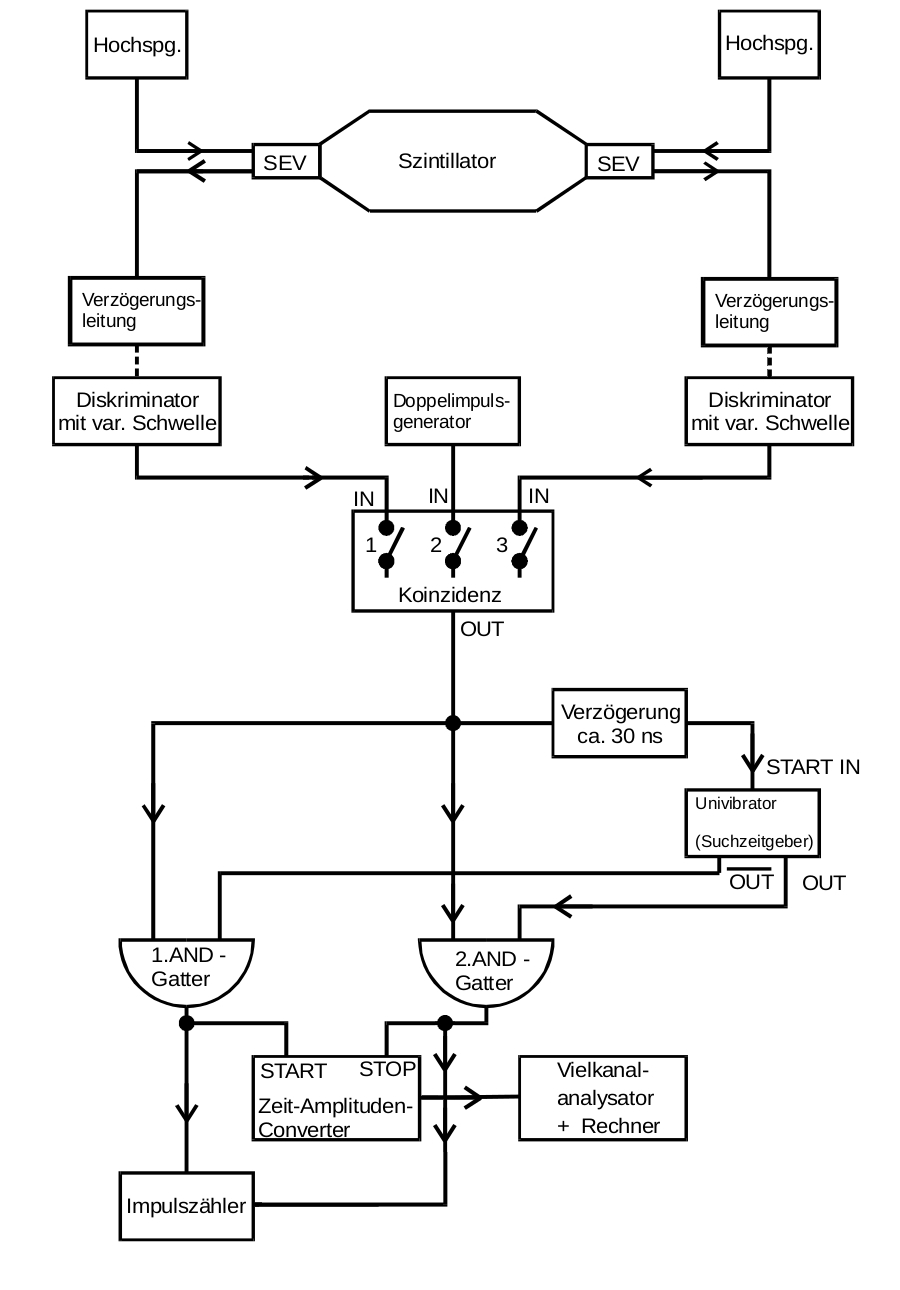
\includegraphics[height=15.5cm]{ressources/aufbau.jpeg}
  \caption{Systematischer Aufbau einer Apparatur, um die Lebensdauer von Myonen zu bestimmen \cite{skript}.}
  \label{fig:aufbau1}
\end{figure}



Die Apparatur besteht aus einem organischen Szintillations-Detektor.
Wenn ein Myon in den Detektor fällt, gibt es seine kinetische Energie an die Moleküle des Szintillatormaterials ab, welche dadurch in einen angeregten Zustand übergehen.
Bei der Rückkehr in den Grundzustand wird dementsprechend ein Lichtimpuls emittiert.
Zerfällt nun das Myon im Szintillator, entsteht ein Elektron, welches, wie zuvor das Myon, seine kinetische Energie an das Szintillatormaterial abgibt.
Es entsteht erneut ein Lichtimpuls.
Der Abstand der beiden Lichtimpulse ist dabei die Individuallebenszeit des Myons.
Die Lichtimpulse werden von Photokathoden in elektrische Signale umgewandelt.
Die daran anschließenden Sekundärelektronenvervielfacher (SEV) verstärken das elektrische Signal.
Da es bei endlicher Temperatur in dem SEV zu thermischer Emission von Elektronen kommen kann, werden zwei SEVs eingesetzt, welche eine Koinzidenz durchlaufen.
Weil diese thermische Emission der beiden SEVs unkorreliert sind, können diese Fehlimpulse durch die Koinzidenz herausgefiltert werden.
Hierbei wird eine Verzögerungsleitung eingesetzt, da die SEVs verschiedene elektronische Eigenschaften besitzen.\\
Die Diskriminatoren erfüllen mehrere Funktionen.
Zunächst wandeln sie das elektrische Signal, welches aus den SEVs kommt, in einen elektrischen Impuls mit fest definierter Breite und Höhe um, der von der Logik des NIM-Standards verarbeitet werden kann.
%Die Breite des Signals bestimmt, welche es durch die Koinzidenz schaffen.
Die Koinzidenz leitet die Signale nur weiter, wenn beiden Signale der Diskriminatoren innerhalb der Auflösezeit $\Delta t_\text{K}$ aufeinandertreffen.
Die Auflösezeit hängt von der Verzögerungsleitung und der Breiten der Signale ab.
Sie sollte größer sein als $\SI{4}{\nano\second}$, dem Fall, in dem ein Lichtimpuls direkt an einer der Photokathoden ausgelöst wird.
Desweiteren lassen die Diskriminatoren nur Impulse durch, welche eine Spannungsschwelle von $U_0$ überschreiten.
Da die Impulse, ausgelöst durch die thermische Emission in den SEVs, in der Regel viel kleiner sind als die, welche von Myonen ausgelöst werden, können somit diese Fehlimpulse zusätzlich herausgefiltert werden.\\
An einem Eingang der Koinzidenz befindet sich aus Justagezwecken ein Doppelimpulsgenerator, welcher ein $\SI{1}{\kilo\hertz}$-Signal in einem in $\SI{0,1}{\micro\second}$-Schritten einstellbaren Abstand aussendet.\\
Auf die Koinzidenz folgt die Logik, welche die Lebensdauer der Myonen misst.
Im Idealfall erzeugt das Myon, welches in den Tank fällt, einen Startimpuls.
Selbiges erzeugt beim Zerfall einen Stop-Impuls.
Der Startimpuls geht an den START-Eingang eines Zeit-Amplituden-Converters (TAC), sowie der Stopimpuls an den STOP-Eingang.
Der TAC gibt einen Impuls aus, dessen Höhe proportional zum Zeitunterschied zwischen Start- und Stopsignal ist.
Dieses Signal wird von einem Vielkanalanalysator zu einem Rechner weitergeleitet.
Das auf dem Rechner vorinstallierte Programm ordnet den Impulses je nach Höhe einen Kanal zu.\\
Das Aussehen der Schaltung resultiert jedoch daher, dass ein Großteil der Myonen den Tank durchquert ohne zu zerfallen.
Daher gäbe es einen Start- aber keinen Stopimpuls.
Um dies zu beheben wird eine Monostabile Kippstufe eingesetzt, welche eine einstellbare Suchzeit $T_S$ besitzt.
Der Ausgang der Koinzidenz wird an die Eingänge zweier UND-Gatter und an den Eingang der monostabilen Kippstufe angeschlossen.
Der inverse Ausgang der Kippstufe wird an das UND-Gatter angeschlossen, dessen Ausgang mit dem START-Eingang des TAC verbunden ist.
Der positive Ausgang geht an das andere UND-Gatter, welches an den STOP-Eingang des TAC geht.
Damit ein Startimpuls den TAC startet, wird eine im Vergleich zur Lebensdauer des Myons sehr kleine Verzögerung vor die Kippstufe geschaltet, sodass das erste UND-Gatter das Startsignal weiterleiten kann.
Mit dem Startsignal wird die Suchzeit $T_S$ der Kippstufe gestartet.
Der TAC kann daher nur gestoppt werden, wenn während der Suchzeit ein zweites Signal auftaucht.
Ist dies nicht der Fall, wird mit dem nächsten Signal der TAC wieder gestartet.
Die Suchzeit sollte größer als die Lebensdauer eines Myons, aber auch sehr viel kleiner sein als der zeitliche Abstand, in dem ein anderes Myon in den Tank fällt.
Es kann jedoch immer passieren, dass sich zwei Myonen im Tank befinden.
Dieses Rauschen ist hinreichend gleichmäßig über alle aufgenomenen Zeitintervalle verteilt und ist abhängig von der Suchzeit, der Messzeit und der Gesamtzahl der Startimpulse.
Daher wird zusätzlich an den Ausgang des ersten UND-Gatters ein Impulszähler zugeschaltet.
